\documentclass[11pt,french]{beamer}

\usepackage{newpxtext,newpxmath} % Or \usepackage{palatino}
\usepackage[utf8]{inputenc}
\usepackage[T1]{fontenc}
\usepackage{mathtools,amssymb,stmaryrd}

\SetSymbolFont{stmry}{bold}{U}{stmry}{m}{n}
\usepackage{babel}
\newcommand*{\retour}{\mathord{\leftarrow}}
\newcommand*{\gauche}{\mathord{\blacktriangleleft}}
\newcommand*{\droite}{\mathord{\blacktriangleright}}
\newcommand*{\entree}{\mathord{\blacksquare}}

\newcommand*{\suppr}{\mathord{\rightarrow}}
\newcommand{\egauche}[1]{\overleftarrow{\mathtt{#1}}}
\newcommand{\edroite}[1]{\overrightarrow{\mathtt{#1}}}


\newcommand*{\Clav}{\ensuremath{\mathsf{Clav}}}
\newcommand*{\Rat}{\ensuremath{\mathsf{Rat}}}
\newcommand*{\Rec}{\ensuremath{\mathsf{Rec}}}
\newcommand*{\Alg}{\ensuremath{\mathsf{Alg}}}
\newcommand*{\Cont}{\ensuremath{\mathsf{Cont}}}

\newcommand*{\MK}{\ensuremath{\mathsf{MK}}}

\newcommand*{\EK}{\ensuremath{\mathsf{EK}}}
\newcommand*{\RK}{\ensuremath{\mathsf{RK}}}
\newcommand*{\REK}{\ensuremath{\mathsf{REK}}}

\newcommand*{\FK}{\ensuremath{\mathsf{FK}}}
\newcommand*{\FEK}{\ensuremath{\mathsf{FEK}}}
\newcommand*{\FRK}{\ensuremath{\mathsf{FRK}}}

\newcommand*{\GK}{\ensuremath{\mathsf{GK}}}
\newcommand*{\GRK}{\ensuremath{\mathsf{GRK}}}
\newcommand*{\GEK}{\ensuremath{\mathsf{GEK}}}

\newcommand*{\FREK}{\ensuremath{\mathsf{FREK}}}
\newcommand*{\GREK}{\ensuremath{\mathsf{GREK}}}
\newcommand*{\BREK}{\ensuremath{\mathsf{BREK}}}

\newcommand*{\QMK}{\ensuremath{\mathsf{QMK}}}
\newcommand*{\QRK}{\ensuremath{\mathsf{QRK}}}
\newcommand*{\QGRK}{\ensuremath{\mathsf{QGRK}}}
\newcommand*{\QFRK}{\ensuremath{\mathsf{QFRK}}}

\newcommand*{\BK}{\ensuremath{\mathsf{BK}}}
\newcommand*{\BRK}{\ensuremath{\mathsf{BRK}}}

\let\touche\mathtt
\let\key\touche

\newcommand*{\conf}[2]{
	\left\langle #1 \middle| #2 \right\rangle
}
\let\config\conf


\newcommand*{\act}[1]{\xrightarrow{#1}}
\newcommand*{\actEff}[1]{\xrightarrow{#1}_{\text{e}}}
\newcommand*{\cdotEff}{\odot} %{\cdot_{\text{e}}}
\usetheme{metropolis}
\metroset{progressbar=frametitle}
\metroset{block=fill}

\renewcommand{\L}{\mathcal{L}}
\renewcommand{\bar}{\overline}
\newcommand{\A}{\mathcal{A}}
\newcommand{\Kinf}{||K||_{\infty}}


\title{Claviers symétriques et à états}
\author[Erwann LOULERGUE]{Erwann LOULERGUE, \texorpdfstring{\\supervisé par Vincent PENELLE et Corto MASCLE}{}}
\date{Juin \& Juillet 2022}
\institute[ENS Paris-Saclay]{Au LaBRI}


\begin{document}

\begin{frame}
	\titlepage
\end{frame}

\begin{frame}{Sommaire}
	\tableofcontents
\end{frame}

\section{Les claviers "habituels"}
\begin{frame}
	\frametitle{Le contexte}
	\begin{center}
		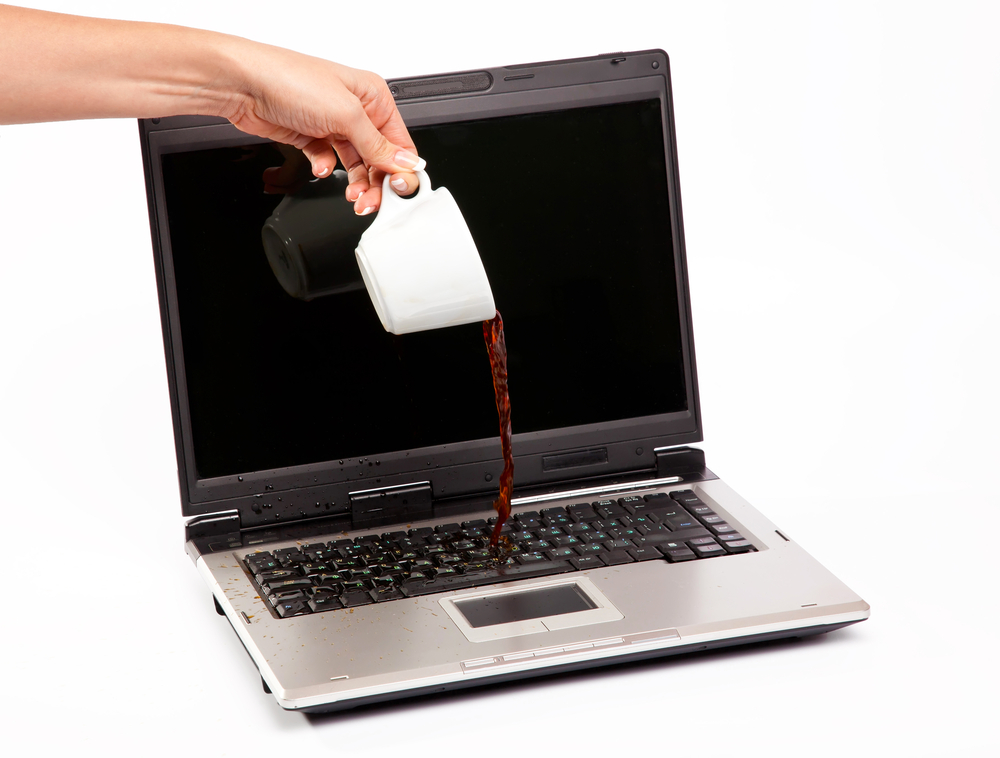
\includegraphics[height=0.3\textwidth]{Drame.jpg}	
	\end{center}

	On possède un clavier ne fonctionnant pas normalement. Par exemple, si on appuie sur la touche $A$, il écrit $\touche{abc}$, si on appuie sur la touche $B$, il efface deux caractères\dots

	Quels mots peut-on écrire avec ce clavier ? Et de manière générale, étant donné un clavier, peut-on écrire un mot donné ?

\end{frame}
\begin{frame}{Définitions}
	\begin{block}{opérations élementaires}
		\begin{itemize}
			\item $\touche{a}$ pour $a \in \Sigma$: écrit "a" à gauche du curseur. \pause
			\item $\retour$: efface la lettre à gauche du curseur. \pause
			\item $\gauche$ et $\droite$: déplace le curseur à gauche ou à droite.
		\end{itemize}
	\end{block}
	On note $S$ l'ensemble des opérations élémentaires.
	\pause
	\begin{block}{Claviers}
		\begin{itemize}
			\item Une \emph{touche} est une suite d'opérations élémentaires. \pause
			\item Un \emph{clavier (automatique)} est un ensemble fini de touches.
		\end{itemize}
	\end{block}
	\begin{exampleblock}{Le clavier précédent}
		Par exemple, le clavier discuté précedemment est $\{\touche{abc},\retour^2\}$
	\end{exampleblock}
\end{frame}

\begin{frame}{Modélisation}
	Quand le mot courant est $uv$ avec le curseur entre $u$ et $v$, on note la configuration $\conf{u}{v}$. \pause

	Les opérations élémentaires induisent des actions sur les configurations :
	\begin{align*}
		\forall a \in A&, \conf{u}{v}\cdot a = \conf{ua}{v} \\
		\conf{\varepsilon}{v}\cdot \retour = \conf{\varepsilon}{v} &, \conf{ua}{v}\cdot \retour = \conf{u}{v} \\
		\conf{\varepsilon}{v}\cdot \gauche = \conf{\varepsilon}{v} &, \conf{ua}{v}\cdot \gauche = \conf{u}{av} \\
		\conf{u}{\varepsilon}\cdot \droite = \conf{u}{\varepsilon} &, \conf{u}{av}\cdot \droite = \conf{ua}{v} \\
	\end{align*}
\end{frame}

\begin{frame}{Modélisation}
	\begin{exampleblock}{Action d'une touche}
		On applique $t = \retour a \droite$ à $\config{c}{d}$. \pause
		 \begin{align*}
			\config{c}{d} & \act{\retour} \config{\varepsilon}{d}\\
						  & \act{a}       \config{a}{d}\\
						  & \act{\droite} \config{ad}{\varepsilon}.
		\end{align*}
		Ainsi $\conf{c}{d}\cdot t = \conf{ad}{\varepsilon}$.
	\end{exampleblock}
	
\end{frame}

\begin{frame}{Les \emph{vrais} claviers} 
	Ces claviers sont assez limités : on n'a pas de notion de saisie qu'on choisirait d'arrêter. \pause On définit donc les \emph{claviers manuels} :
    \begin{block}{Clavier (manuel)}
        Un clavier manuel, ou simplement \textbf{clavier}, est un couple $(T,F)$ d'ensembles finis de touches.
        Une exécution acceptante d'un clavier est une suite de touches de $T$ suivie d'une touche de $F$.
    \end{block} \pause
	\begin{exampleblock}{Remarque}
		Le fait qu'une touche soit finale peut être modélisé par une touche entrée qu'on notera $\entree$.
	\end{exampleblock}
\end{frame}

\begin{frame}{Le langage d'un clavier}
	Pour les claviers automatiques, on a \[\L(K) = \{w | w =uv, \exists t_1...t_n, \conf{\varepsilon}{\varepsilon}\cdot t_1...t_n = \conf{u}{v}\}\] \pause
    Sinon, dans le cas général, on définit $\L(K)$ comme \[\{w | w =uv, \exists t_1...t_n, \conf{\varepsilon}{\varepsilon}\cdot t_1...t_n = \conf{u}{v}, \mathrm{seule~} t_n \mathrm{~est~finale}\}\]
\end{frame}


\begin{frame}
	\frametitle{Classes de claviers}
	\[
	 \begin{array}{cc}
		\mathsf{R}:  \retour & \mathsf{E}:  \entree \\
        \mathsf{G}:  \gauche & \mathsf{F}:  \droite + \gauche \\
	 \end{array}
	\]

	\[
		\begin{array}{ccc}
			\MK : \{\} & \GK : \{\gauche\} & \FK :\{\gauche,\droite\} \\
			\EK : \{\entree\} & \GEK : \{\gauche,\entree\} & \FEK :\{\gauche,\droite,\entree\} \\
			\RK : \{\retour\} & \GRK : \{\gauche,\retour\} & \FRK :\{\gauche,\droite,\retour\} \\
			\REK : \{\retour, \entree\} & \GREK : \{\gauche,\retour,\entree\} & \FREK :\{\gauche,\droite,\retour,\entree\} \\
		\end{array}
	\]
 \end{frame}


\section{Claviers à états}
\begin{frame}{Définition}
	\begin{block}{Clavier à état}
		Un clavier à états est la donnée de $(Q,\Delta ,F,s_0)$ où :
        \begin{itemize}
            \item $Q$ est un ensemble d'\textbf{états}
            \item $\Delta \subset Q \times S^* \times Q$ est un ensemble fini de \textbf{transitions}
            \item $F$ est un ensemble d'états dits \textbf{finaux}
            \item $s_0 \in Q$ est un état dit \textbf{initial}
        \end{itemize}
	\end{block}
	\pause
	\begin{block}{Configuration étatique}
		La configuration d'un clavier à états pendant son calcul est décrite par $(u,q,v) \in A^* \times Q \times A^*$, appelé \textbf{configuration étatique}.
	\end{block}
\end{frame}
\begin{frame}{Définition}
	\begin{block}{Clavier à état}
		Un clavier à états est la donnée de $(Q,\Delta ,F,s_0)$
	\end{block}

	\begin{block}{Configuration étatique}
		La configuration d'un clavier à états pendant son calcul est décrite par $(u,q,v) \in A^* \times Q \times A^*$, appelé \textbf{configuration étatique}.
	\end{block}
	\begin{exampleblock}{Action d'une touche sur une configuration}	
		Soit $(u,q,v)$ une configuration étatique, et $(q,t,q') \in \Delta$. En appliquant cette transition, on passe dans la configuration $(u',q',v')$, avec $\conf{u'}{v'} = \conf{u}{v} \cdot t$.
	\end{exampleblock}
\end{frame}
\end{document}